%
% Niniejszy plik stanowi przykład formatowania pracy magisterskiej na
% Wydziale MIM UW.  Szkielet użytych poleceń można wykorzystywać do
% woli, np. formatujac wlasna prace.
%
% Zawartosc merytoryczna stanowi oryginalnosiagniecie
% naukowosciowe Marcina Wolinskiego.  Wszelkie prawa zastrzeżone.
%
% Copyright (c) 2001 by Marcin Woliński <M.Wolinski@gust.org.pl>
% Poprawki spowodowane zmianami przepisów - Marcin Szczuka, 1.10.2004
% Poprawki spowodowane zmianami przepisow i ujednolicenie 
% - Seweryn Karłowicz, 05.05.2006
% Dodanie wielu autorów i tłumaczenia na angielski - Kuba Pochrybniak, 29.11.2016

% dodaj opcję [licencjacka] dla pracy licencjackiej
% dodaj opcję [en] dla wersji angielskiej (mogą być obie: [licencjacka,en])
\documentclass[licencjacka]{pracamgr}


% Dane magistranta:
\autor{Michał Izworski}{360968}


% Dane magistrantów:
%\autor{Autor Zerowy}{342007}
%\autori{Autor Pierwszy}{342013}
%\autorii{Drugi Autor-Z-Rzędu}{231023}
%\autoriii{Trzeci z Autorów}{777321}
%\autoriv{Autor nr Cztery}{432145}
%\autorv{Autor nr Pięć}{342011}

\title{AlphaSoccer: gra w ,,Piłkarzyki~na~kartce'' za pomocą głębokich sieci neuronowych}


%\tytulang{An implementation of a difference blabalizer based on the theory of $\sigma$ -- $\rho$ phetors}

%kierunek: 
% - matematyka, informacyka, ...
% - Mathematics, Computer Science, ...
\kierunek{Międzykierunkowe Studia Ekonomiczno-Matematyczne}

% informatyka - nie okreslamy zakresu (opcja zakomentowana)
% matematyka - zakres moze pozostac nieokreslony,
% a jesli ma byc okreslony dla pracy mgr,
% to przyjmuje jedna z wartosci:
% {metod matematycznych w finansach}
% {metod matematycznych w ubezpieczeniach}
% {matematyki stosowanej}
% {nauczania matematyki}
% Dla pracy licencjackiej mamy natomiast
% mozliwosc wpisania takiej wartosci zakresu:
% {Jednoczesnych Studiow Ekonomiczno--Matematycznych}

% \zakres{Tu wpisac, jesli trzeba, jedna z opcji podanych wyzej}

% Praca wykonana pod kierunkiem:
% (podać tytuł/stopień imię i nazwisko opiekuna
% Instytut
% ew. Wydział ew. Uczelnia (jeżeli nie MIM UW))
\opiekun{prof. dr hab. Andrzej Skowron\\
  Wydział Matematyki, Informatyki i Mechaniki\\
  }

% miesiąc i~rok:
\date{Czerwiec 2018}

%Podać dziedzinę wg klasyfikacji Socrates-Erasmus:
\dziedzina{ 
%11.0 Matematyka, Informatyka:\\ 
%11.1 Matematyka\\ 
%11.2 Statystyka\\ 
%11.3 Informatyka\\ 
11.4 Sztuczna inteligencja\\ 
%11.5 Nauki aktuarialne\\
%11.9 Inne nauki matematyczne i informatyczne
}

%Klasyfikacja tematyczna wedlug AMS (matematyka) lub ACM (informatyka)
\klasyfikacja{Computing methodologies\\
	Machine learning\\
 	Learning paradigms\\
	Reinforcement learning\\
	Sequential decision making}

% Słowa kluczowe:
\keywords{machine learning, reinforcement learning, deep learning, actor-critic methods, monte carlo tree search}

% Tu jest dobre miejsce na Twoje własne makra i~środowiska:
\newtheorem{defi}{Definicja}[section]
\usepackage{wrapfig}
\usepackage{graphicx}
\graphicspath{ {img/} }
\usepackage{amsfonts}
\usepackage{amsmath}
\usepackage{algorithm}
\usepackage[noend]{algpseudocode}


\makeatletter
\def\BState{\State\hskip-\ALG@thistlm}
\makeatother

% koniec definicji

\begin{document}

\maketitle

%tu idzie streszczenie na strone poczatkowa
\begin{abstract}
  TO DO
\end{abstract}

\tableofcontents
%\listoffigures
%\listoftables

\chapter{Wprowadzenie}\label{r:intro}

%Sztuczna inteligencja cieszy się ogromnym wzrostem zainteresowania w ostatnim czasie, zarówno wśród społeczności naukowej, jak i w przemyśle. Swoją popularność zawdzięcza temu, iż dzięki niej jesteśmy w stanie poradzić sobie z problemami, których rozwiązania przy użyciu programów komputerowych przynosiły bardzo mierne rezultaty. 
%Na szczególną uwagę zasługuje Uczenie Maszynowe (ang. Machine Learning), które jest obecnie wiodącym nurtem i przyciąga największą uwagę ze względu na najlepsze rezultaty.
%Pozwoliło nam ono na tworzenie programów do rozpoznawania obrazów, tłumaczenia maszynowego czy generowania muzyki. 
%Sztuczna inteligencja okazała się 

%Uczenie Maszynowe cieszy się ogromnym wzrostem zainteresowania w ostatnim czasie, zarówno wśród społeczności naukowej, jak i w przemyśle.
%Pozwoliło nam ono na rozwiązanie problemów, których wcześniejsze próby rozwiązania dawały kiepskie rezultaty, takich jak rozpoznawania obrazów, tłumaczenia maszynowego czy generowania muzyki.
%Jednym z przełomowych wyników sztucznej inteligencji, jakie udało nam się uzyskać

%\section{Intro}

Interakcja z otoczeniem jest prawdopodobnie dla większości z nas naturalnym sposobem uczenia się. 
Dziecko uczące się stawiać pierwsze kroki nie posiada nauczyciela, który dokładnie instruuje je w jaki sposób powinno układać nogi, aby zachować równowagę. 
Zamiast tego, poprzez metodę prób i błędów, stara się ono zrozumieć w jaki sposób zrealizować swój cel i poznaje jakie efekty przynosi wykonywanie przez nie konkretnych ruchów. 
W ten sam sposób uczymy się przez całe życie, jednocześnie poznając otaczający nas świat oraz prawa, które nim rządzą, bez względu na to czy jest to nauka jazdy samochodem czy gry w szachy.

%\section{Intro2}

\section{Piłkarzyki na kartce}

Piłkarzyki na kartce to gra strategiczna, odbywającą się na prostokątnym boisku, rysowanym zazwyczaj na kartce w kratę.
Gracze na przemian wykonują ruchy polegające na przemieszczeniu piłki na sąsiednie pola, aż znajdzie się ona w jednej z bramek lub nie będzie możliwe wykonanie kolejnego ruchu.

\begin{figure}[ht]
  \centering
  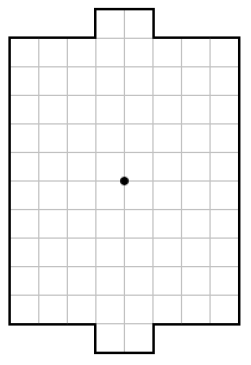
\includegraphics[width=0.2\textwidth]{board}
  \caption{Pusta plansza}
\end{figure}

Najczęściej stosowanym wymiarem planszy jest 8x10 kratek.
Przy krótszych bokach narysowane są dwie bramki o szerokości 2 kratek, w których gracze muszą umieścić piłkę.
Rozgrywka toczy się jedynie na przecięciach linii.
Środek planszy jest punktem startowym gry, do którego gracze dorysowują kolejne linie, oznaczające przemieszczenie piłki na sąsiednie pole. Każdy kolejny ruch zaczyna się w miejscu, w którym skończył się poprzedni, wzdłuż kratki lub po przekątnej. 

Ruchy nie mogą odbywać się po brzegu planszy ani wzdłuż odcinków, po których wcześniej piłka była już prowadzona.
Możliwe jest odbijanie się, które polega na wykonaniu przez gracza dodatkowego ruchu. Następuje ono gdy ruch zostanie zakończony w miejscu, w którym kończy się już linia narysowana przez jednego z graczy lub na brzegu boiska. 

\begin{figure}[ht]
  \centering
  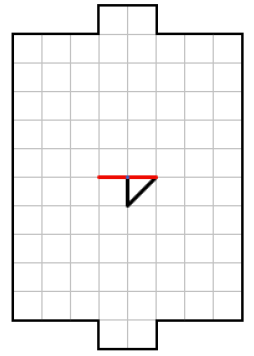
\includegraphics[width=0.2\textwidth]{odbicie}
  \caption{Odbicie (kolor czerwony)}
\end{figure}

Gra kończy się w momencie gdy piłka znajdzie się w jednej z bramek.
Wówczas gracz, do którego należy dana bramka, przegrywa. 
Gracz może również przegrać w wypadku gdy nie jest w stanie wykonać żadnego ruchu.


\begin{figure}[ht]
  \centering
  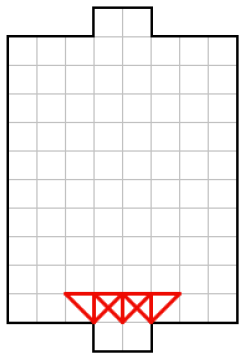
\includegraphics[width=0.2\textwidth]{zablokowanie}
  \caption{Zablokowana bramka}
\end{figure}
 
\chapter{Uczenie ze Wzmocnieniem}\label{r:rl}

\section{Wprowadzenie}

Uczenie ze wzmocnieniem (ang. Reinforcement Learning, RL) jest działem uczenia maszynowego, zajmującym się sekwencyjnym podejmowaniem decyzji. Na proces uczenia składa się \emph{agent}, który uczy się podejmować decyzje oraz \emph{środowisko}, które stanowi cały świat zewnętrzy dla agenta. Interakcja między nimi polega na naprzemiennym wykonywaniu akcji przez agenta oraz prezentowaniu nowej sytuacji, w której on się znalazł i nagrody jaką otrzymał przez środowisko. Celem agenta jest maksymalizacja nagród, które otrzymuje.
Podczas procesu uczenia się, nigdy nie wskazujemy agentowi którą akcje powinien on wykonać, co stanowi główną różnice pomiędzy uczeniem ze wzmocnieniem a uczeniem nadzorowanym (ang. Supervised Learning). 

\section{Dyskretny Proces Markowa}

Dyskretny Proces Markowa składa się z:
\begin{itemize}
\item zbioru stanów w których może znaleźć się agent, $ s \in \mathcal{S} $,
\item rozkładu stanu początkowego $\mathcal{D}$ nad zbiorem $\mathcal{S}$,
\item zbioru akcji możliwych do podjęcia przez agenta, $ a \in \mathcal{A} $
\item nagrody otrzymywanej przez agenta za każdym razem, gdy ten wykona jakąś akcje, $ r_t \in \mathbb{R} $
\item prawdopodobieństwa przejścia między stanami
$$ p(s'|s, a) = \mathbb{P}(s_{t+1} = s' \mid s_t = s, a_t = a)$$
\item funkcji nagrody, $ R : S \times S \times A \rightarrow \mathbb{R} $
$$ R(s, a, s') = \mathbb{E}(r_{t+1} \mid s_t = s, a_t = a, s_{t+1} = s') $$
\item współczynnik dyskontującego wartości nagród otrzymywanych w przyszłości $ \gamma \in [0, 1] $
\end{itemize}


\section{Wynik oraz epizody}

Interakcja między agentem a środowiskiem zachodzi w każdym, dyskretnym punkcie czasu $ t = 0, 1, 2, ... $. Znajdując się w punkcie czasu $t$, agent obserwuje stan $ s_t \in \mathcal{S} $, w którym się znajduję, na jego podstawie wykonuje akcję $ a_t \in \mathcal{A}(s) $, gdzie $ \mathcal{A}(s) $ jest zbiorem wszystkich akcji, które można wykonać znajdując się w stanie $s$. W kolejnym kroku dowiaduje się on jaką nagrodę $ r_{t+1} \in \mathbb{R} $ otrzymał i do jakiego stanu $ s_t{t+1} $ się przeniósł. W wyniku otrzymujemy następujący ciąg stanów, akcji oraz nagród, zwany \emph{trajektorią}:

$$ s_0, a_0, r_1, s_1, a_1, r_2, ... $$


\begin{figure}[ht]
  \centering
  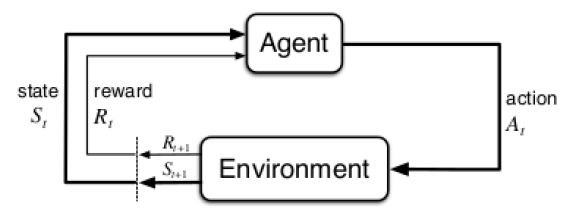
\includegraphics[width=0.5\textwidth]{agent_env_interaction}
  \caption{Interakcja między agentem a środowiskiem jako Dyskretny Proces Markowa}
\end{figure}

Najprostszym typem środowisk są te w których ilość kroków jest z góry ograniczona. Pojedynczy ciąg interakcji nazywamy wówczas \emph{epizodem}, a ostatni stan obserwowany przez agenta -- \emph{stanem terminalnym}. W tym wypadku epizody są od siebie niezależne, mogą się one kończyć w różnych stanach oraz po różnej ilości kroków. 

Celem naszego agenta jest maksymalizacja wartości oczekiwanej sumy nagród, które zdobędzie on w przyszłości. Określmy ją jako \emph{wynik}, $ G_t $, który zdefiniowany jest następująco:

$$ G_t = r_{t+1} + r_{t+2} + r_{t+3} + ... + r_{T-1} = r_{t+1} + G_{t+1} $$

gdzie $T$ jest końcem epizodu, a $t$ indeksem czasu. Sam problem nauczenia naszego agenta w jaki sposób powinien on podejmować decyzje, aby osiągnąć najwyższy wynik, nazywamy \emph{epizodycznym zadaniem}.

Możemy również spotkać się ze środowiskami, z którymi interakcja przebiega nieprzerwanie. Mamy wówczas do czynienia z \emph{ciągłym zadaniem}. Wprowadzamy wówczas koncepcje \emph{dyskontowania} wyniku, który definiujemy następująco:

$$ G_t = r_{t+1} + \gamma r_{t+2} + \gamma^2 r_{t+3} + ... = 
\sum_{k=0}^{\infty} \gamma^k r_{t+k+1} $$

gdzie $ \gamma \in [0, 1) $.


\section{Polityka}

Polityka jest funkcją która każdemu stanowi przyporządkowuje akcję. Może być ona deterministyczna, $ \pi(s) $, bądź też stochastyczna, $ \pi(a \mid s) $, i wówczas stanowić rozkład prawdopodobieństwa wszystkich akcji dla ustalonego stanu. Metody uczenia ze wzmocnieniem określają w jaki sposób polityka jest modyfikowana na podstawie doświadczenia zbieranego przez agenta.

\section{Funkcja Wartości}

Posiadając już politykę naszego agenta, możemy chcieć się dowiedzieć jaką nagrodę uzyska agent, który będzie jej przestrzegał. W tym celu definiujemy \emph{funkcję wartości stanu} (ang. Value Function), którą oznaczamy jako $ v_{\pi}(s) $ dla ustalonej polityki $ \pi $. Definiujemy ją jako:

$$ v_{\pi}(s) = \mathbb{E}_{\pi}[G_t \mid S_t = s] = \mathbb{E}_{\pi} \Bigg[ \sum_{k=0}^{\infty} \gamma^k R_{t+k+1} \bigg| S_t = s \Bigg] $$

gdzie $ \mathbb{E}_{\pi} $ jest wartością oczekiwaną przy założeniu że agent kieruje się polityką $\pi$, z kolei $t$ jest dowolnym punktem w czasie. 

Podobnie definiujemy wartość wybrania akcji $a$, gdy znajdujemy się w stanie $s$ oraz podążamy zgodnie z polityką $\pi$, oznaczaną jako $q_{\pi}(s, a)$. Jest ona wartością oczekiwaną z sytuacji w której rozpoczynamy w stanie $s$, wykonujemy akcję $a$, po czym wszystkie kolejne akcje wykonujemy zgodnie z polityką $\pi$. Funkcję tę nazywamy \emph{funkcją wartości akcji}.

$$ q_{\pi}(s, a) = \mathbb{E}_{\pi}[G_t \mid S_t = s, A_t = a] = \mathbb{E}_{\pi} \Bigg[ \sum_{k=0}^{\infty} \gamma^k R_{t+k+1} \bigg| S_t = s, A_t = a \Bigg] $$

\section{Optymalność polityki oraz funkcji wartości}

Podczas rozwiązywania problemu uczenia ze wzmocnieniem staramy się znaleźć politykę, której przestrzeganie przyniesie naszemu agentowi jak największą nagrodę. Będziemy mówić że polityka $\pi$ jest lepsza lub równa polityce $\pi'$, wtedy i tylko wtedy gdy oczekiwana nagroda dla niej jest większa lub równa niż dla $\pi'$ w każdym stanie należącym do przestrzeni stanów. Zawsze istnieje polityka, która jest lepsza lub równa od wszystkich innych i nazywamy ją \emph{optymalną polityką}. Może istnieć wiele różnych od siebie optymalnych polityk, jednak każdą z nich oznaczamy jako $\pi_{\ast}$. Dla wszystkich z nich funkcja wartości stanu jest taka sama i nazywamy ją \emph{optymalną funkcją wartości stanu}. Spełnia ona własność:

$$ v_{\ast}(s) = \max_{\pi} v_{\pi}(s) $$

dla każdego stanu $s \in \mathcal{S}$. Podobnie współdzielą one \emph{optymalną funkcję wartości akcji}, $q_{\ast}$, która spełnia:

$$ q_{\ast}(s, a) = \max_{\pi} q_{\pi}(s, a) $$

dla każdego stanu $s \in \mathcal{S}$ oraz akcji $a \in \mathcal{A}$.

Ponadto optymalną funkcję wartości stanu możemy zdefiniować odwołując się do funkcji wartości akcji w następujący sposób:

$$ v_{\ast}(s) = \max_{a \in \mathcal{A}} q_{\pi_{\ast}}(s) $$

Podstawową własnością, jaką spełniają funkcje wartości, jest \emph{równanie Bellmana}. Dla dowolnej polityki $\pi$ oraz stanu $s$ zachodzi:

\begin{align}
v_{\pi}(s) &= \mathbb{E}_{\pi}[G_t \mid S_t = s]  \nonumber \\
&= \mathbb{E}_{\pi}[r_{t+1} + \gamma G_{t+1} \mid S_t = s] \nonumber \\
&= \sum_a \pi(a \mid s) \sum_s' \sum_r p(s', r \mid s, a) \Big[r + \gamma \mathbb{E}_{\pi}[G_{t+1} \mid S_{t+1} = s' ]\Big] \nonumber \\
&= \sum_a \pi(a \mid s) \sum_{s', r} p(s', r \mid s, a) \Big[r + \gamma v_{\pi}(s') \Big]
\end{align}

Na podstawie własności optymalnych funkcji wartości oraz równania Bellmana możemy wyprowadzić \emph{równania optymalności Bellmana}, bez odwoływania się przy tym do żadnej polityki. Pierwsze z nich odnosi się do funkcji wartości stanu:

\begin{align}
v_{\ast}(s) &= \max_{a \in \mathcal{A}} q_{\pi_{\ast}}(s, a) \nonumber \\
&= \max_a \mathbb{E}_{\pi}[G_t \mid S_t = s, A_t = a]  \nonumber \\
&= \max_a \mathbb{E}_{\pi}[r_{t+1} + \gamma G_{t+1} \mid S_t = s, A_t = a] \nonumber \\
&= \max_a \mathbb{E}[r_{t+1} + \gamma v_{\pi_{\ast}}(S_{t+1}) \mid S_t = s, A_t = a] \nonumber \\
&= \max_a \sum_{s', r} p(s', r \mid s, a) \Big[r + \gamma v_{\ast}(s') \Big]
\end{align}

Natomiast drugie zdefiniowane jest dla funkcji wartości akcji:

\begin{align}
q_{\ast}(s, a) &= \mathbb{E}[r_{t+1} + \gamma \max_{a'} q_{\ast} (S_{t+1}, a') \mid S_t = s, A_t = a] \nonumber \\
&= \sum_{s', r} p(s', r \mid s, a) \Big[r + \gamma \max_{a'} q_{\ast} (s', a') \Big]
\end{align}

\section{Metody uczenia ze wzmocnieniem}

Metody rozwiązywania problemu uczenia ze wzmocnieniem możemy podzielić ze względu na to, czy wykorzystują one model środowiska. Metody \emph{model-based} wymagają od nas \emph{modelu} środowiska, z którego nasz agent będzie korzystał podczas aby przewidzieć w jaki sposób środowisko będzie zachowywało się w odpowiedzi na wykonywane przez niego akcje.
Dzięki temu możliwe jest \emph{planowanie}, które pozwala na przewidywanie zachowania środowiska wiele kroków wprzód. Tego typu problemy możemy spotkać przy okazji nauki naszego agenta w Go, gdzie środowisko imitowane jest przez niego samego, podczas gdy gra on sam ze sobą. 
Drugą klasą algorytmów są metody \emph{model-free}, w których agent posiada jedynie politykę oraz funkcję wartości, a samo zachowanie środowiska jest dla niego nieznane i może on obserwować jedynie bezpośrednie skutki swoich działań. Z takimi problemami spotykamy się np. w przypadku gry naszego agenta na Atari, gdzie nie próbujemy dowiedzieć się jakie prawa rządzą poszczególnymi grami, a zamiast tego po prostu dajemy naszemu agentowi grać.

\subsection{Metody Monte Carlo}

Metody Monte Carlo korzystają z idei \emph{uogólnionej iteracji polityki}, która składa się z dwóch, przeplatających się ze sobą procesów. Pierwszy krok, nazywany \emph{krokiem ewaluacji polityki}, polega na aproksymacji funkcji wartości na podstawie polityki, wykorzystywanej przez agenta. Z kolei w drugim kroku ulepszamy obecną politykę, przy użyciu wcześniej uzyskanej funkcji wartości. Nazywamy go \emph{krokiem ulepszania polityki}.

W przypadku metod Monte Carlo, ewaluacje polityki wykonujemy poprzez próbkowanie kolejnych trajektorii, a następnie wyliczanie średniego wyniku dla każdego ze stanów, bądź każdej pary stan-akcja. Zbierana przez nas historia akcji w postaci trajektorii nazywamy \emph{doświadczeniem} agenta. Najprostszy sposób aktualizacji funkcji wartości może wyglądać następująco:

$$ v(s_t) \leftarrow v(s_t) + \alpha \big[G_t - v(s_t)\big] $$

gdzie $G_t$ oznacza wynik agenta następujący po czasie $t$, a $\alpha$ parametrem wpływającym na szybkość uczenia się.

Ulepszanie polityki następuje poprzez zachłanny wybór najlepszej akcji dla każdego ze stanów, przy pomocy funkcji wartości akcji. Jednak w przypadku takiego doboru polityki, skazujemy się na deterministyczną politykę, która nie jest w stanie odkrywać nowych, potencjalnie lepszych akcji, gdyż cały czas wybierać będzie ona te same akcje. 

Aby utrzymać eksploracje nowych akcji oraz stanów, wprowadzamy pojęcie \emph{$\epsilon$--zachłannej} polityki, która z wysokim prawdopodobieństwem wykonuje akcję, która maksymalizuje wartość funkcji wartości akcji, a od czasu do czasu wykonuje losową akcję. Dzięki temu utrzymujemy stały poziom eksploracji, a przy niewielkich założeniach dla epsilona polityka zbiega do optymalnej.

$$
\pi(a \mid s) =
\begin{cases}
    1 - \epsilon + \epsilon/\lvert \mathcal{A}(s) \rvert & \text{if } a = a^\ast \\
    \epsilon/\lvert \mathcal{A}(s),              & \text{if } a\neq a^\ast
\end{cases}
$$

Metody Monte Carlo cierpią z powodu wysokiej wariancji podczas uczenia, przez co potrzeba bardzo wielu iteracji, aby agent mógł wyuczyć się sensownej polityki. Są one przykładem metod model-free.

\subsection{Temporal-Difference Learning} 

Prawdopodobnie najważniejszą ideą wykorzystywaną  w uczeniu ze wzmocnieniem jest \emph{temporal-difference} (TD) learning. Podobnie do metod Monte Carlo wykorzystuje ono doświadczenie agenta, bez użycia modelu środowiska. Nie jest wymagane jednak oczekiwanie na zakończenie epizodu, aby zaktualizować wartość funkcji wartości, a zamiast tego aktualizacje mogą następować po wykonaniu pojedynczego kroku. Aktualizacja funkcji wartości w przypadku TD learning może wyglądać następująco:

$$ V(S_t) \leftarrow V(S_t) + \alpha \big[R_{t+1} + \gamma V(S_{t+1}) - V(S_t) \big] $$

Sposób tej aktualizacji nazywany jest \emph{TD(0)} lub też \emph{jedno--krokowym} TD, a sam wyraz o który aktualizowana jest wartość:

$$ \delta_t = R_{t+1} + \gamma V(S_{t+1}) - V(S_t) $$

nazywamy \emph{błędem TD}.

\begin{figure}[ht]
  \centering
  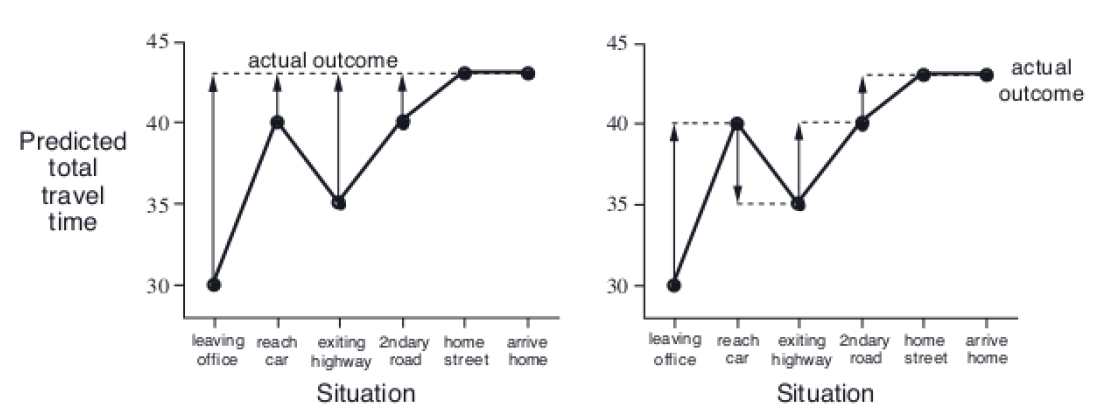
\includegraphics[width=1.0\textwidth]{mc_td}
  \caption{Porównanie aktualizacji funkcji wartości w przypadku metod Monte Carlo (po lewej) oraz metod TD (po prawej)}
\end{figure}

Metody w uczeniu ze wzmocnieniem dzielimy również ze względu na to czy ewaluacja polityki przebiega przy użyciu polityki, która została wykorzystana podczas generowania trajektorii. Metody ewaluujące tę samą politykę nazywamy \emph{on-policy}, natomiast te które działają na różnych politykach nazywamy \emph{off-policy}.

Dwoma podstawowymi algorytmami zaliczającymi się do TD learning jest \emph{SARSA (State-Action-Reward-State-Action} oraz \emph{Q-Learning}.

SARSA jest przykładem metody on-policy, która wykorzystuje funkcję wartości akcji, zamiast funkcji wartości stanu. Algorytm aktualizacji funkcji wartości oraz wyboru polityki wygląda następująco:

\begin{algorithm}
\caption{SARSA}\label{sarsa}
\begin{algorithmic}[1]
\State $\textit{Zainicjalizuj } Q(s, a) \textit{ losowo oraz } Q(\textit{\emph{stan-terminalny}}, \cdot ) = 0$

\Repeat $ \textit{ (dla każdego epizodu)} $
\State $\textit{Zainicjalizuj } S$
\State $\textit{Wybierz akcję A dla stanu S korzystając z polityki pochodzącej z Q (np. } \epsilon \textit{-zachłanną)} $

\Repeat $\textit{ (dla każdego kroku w epizodzie)} $

\State $ \textit{Wykonaj akcję A, zaobserwuj R, S'} $
\State $ \textit{Wybierz akcję A' dla stanu S' korzystając z polityki pochodzącej z Q (np. } \epsilon \textit{-zachłanną)} $
\State $ Q(S, A) \gets Q(S,A) + \alpha \big[ R + \gamma Q(S', A') - Q(S, A) \big] $
\State $ S \gets S'; A \gets A'; $

\Until $ S \textit{ jest stanem terminalnym} $

\Until $ \textit{(koniec epizodów)}$ 
\end{algorithmic}
\end{algorithm}

\section{Podsumowanie}

\chapter{Głębokie Sieci Neuronowe}

\chapter{Głębokie Uczenie ze Wzmocnieniem}

\chapter{Gra w piłkarzyki na kartce}

\chapter{Wnioski}

\begin{thebibliography}{99}
\addcontentsline{toc}{chapter}{Bibliografia}

\bibitem[Bea65]{beaman} Juliusz Beaman, \textit{Morbidity of the Jolly
    function}, Mathematica Absurdica, 117 (1965) 338--9.

\bibitem[Blar16]{eb1} Elizjusz Blarbarucki, \textit{O pewnych
    aspektach pewnych aspektów}, Astrolog Polski, Zeszyt 16, Warszawa
  1916.

\bibitem[Fif00]{ffgg} Filigran Fifak, Gizbert Gryzogrzechotalski,
  \textit{O blabalii fetorycznej}, Materiały Konferencji Euroblabal
  2000.

\bibitem[Fif01]{ff-sr} Filigran Fifak, \textit{O fetorach
    $\sigma$-$\rho$}, Acta Fetorica, 2001.

\bibitem[Głomb04]{grglo} Gryzybór Głombaski, \textit{Parazytonikacja
    blabiczna fetorów --- nowa teoria wszystkiego}, Warszawa 1904.

\bibitem[Hopp96]{hopp} Claude Hopper, \textit{On some $\Pi$-hedral
    surfaces in quasi-quasi space}, Omnius University Press, 1996.

\bibitem[Leuk00]{leuk} Lechoslav Leukocyt, \textit{Oval mappings ab ovo},
  Materiały Białostockiej Konferencji Hodowców Drobiu, 2000.

\bibitem[Rozk93]{JR} Josip A.~Rozkosza, \textit{O pewnych własnościach
    pewnych funkcji}, Północnopomorski Dziennik Matematyczny 63491
  (1993).

\bibitem[Spy59]{spyrpt} Mrowclaw Spyrpt, \textit{A matrix is a matrix
    is a matrix}, Mat. Zburp., 91 (1959) 28--35.

\bibitem[Sri64]{srinis} Rajagopalachari Sriniswamiramanathan,
  \textit{Some expansions on the Flausgloten Theorem on locally
    congested lutches}, J. Math.  Soc., North Bombay, 13 (1964) 72--6.

\bibitem[Whi25]{russell} Alfred N. Whitehead, Bertrand Russell,
  \textit{Principia Mathematica}, Cambridge University Press, 1925.

\bibitem[Zen69]{heu} Zenon Zenon, \textit{Użyteczne heurystyki
    w~blabalizie}, Młody Technik, nr~11, 1969.

\end{thebibliography}

\end{document}


%%% Local Variables:
%%% mode: latex
%%% TeX-master: t
%%% coding: latin-2
%%% End:
